\documentclass{article}
%
% Demo of the mcode package from 
% http://www.mathworks.co.uk/matlabcentral/fileexchange/8015-m-code-latex-package
% Updated 06 Mar 2014
%

\usepackage{graphicx}
\usepackage{wrapfig}
\usepackage{mathtools}
\usepackage{mathrsfs}
\usepackage{enumitem}
\usepackage{pdflscape}
\usepackage{color}
\usepackage{float}
\usepackage{amssymb}

\graphicspath{ {images/} }

% load package with ``framed'' and ``numbered'' option.
\usepackage[framed,numbered,autolinebreaks,useliterate]{mcode}

% something NOT relevant to the usage of the package.
\usepackage{url}
\setlength{\parindent}{0pt}
\setlength{\parskip}{18pt}


% //////////////////////////////////////////////////

\begin{document}

\title{Homework 7 - Optimal Control Systems}
\author{Erivelton Gualter dos Santos, 2703806}
\date{}

\maketitle 

\section{Zermelo's problem}

\begin{itemize}
\item In order to reach the final condition, it was solved the zermelo's problem for the initial angle from $0$ to $2\pi$ with a step size of $0.001$. Therefore, the best initial condition angle was chosen according to the minimum euclidean distance to final position.
\item Then,  using the numerically solver ``vpasolve" to find the solution for the following equation with the initial guess found previously, it reached the position in $5.4435$ s.
\begin{equation*}
x = -\frac{1}{2}\left[\sec\theta_f(\tan\theta_f - \tan\theta) - \tan\theta_f(\sec\theta_f-sec\theta)+\ln\left(\frac{\tan\theta_f+\sec\theta_f}{\tan\theta+\sec\theta} \right) \right]
\end{equation*}
\end{itemize}

\begin{figure}[H]
\centering
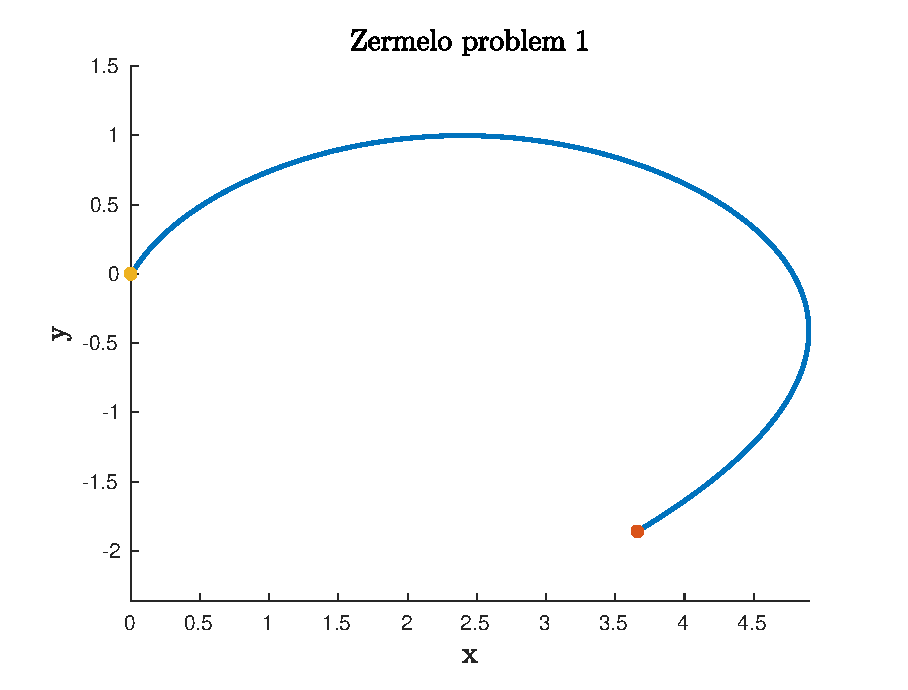
\includegraphics [width=3.5in]{f1}
\caption{Zermelo's solution for x(0) = 3.66, y(0) = -1.86 }
\end{figure}

\section{Zermelo's problem}

\begin{itemize}
\item As in the problem 1, it was performed an interaction guess for the angle from $0$ to $2\pi$ with a step size of $0.001$. 
\item Consequently, it was used the numerically solver to found $\theta$ and $\theta_f$ using the previously value as a guess.
\begin{equation*}
x = -\frac{1}{2}\left[\csc\theta_f(\cot\theta_f - \cot\theta) - \cot\theta_f(\csc\theta_f-csc\theta)+\ln\left(\frac{\cot\theta_f+\csc\theta_f}{\cot\theta+\csc\theta} \right) \right]
\end{equation*}
\item The duration time to reach the final position is $4.0785$ s.
\end{itemize}

\begin{figure}[H]
\centering
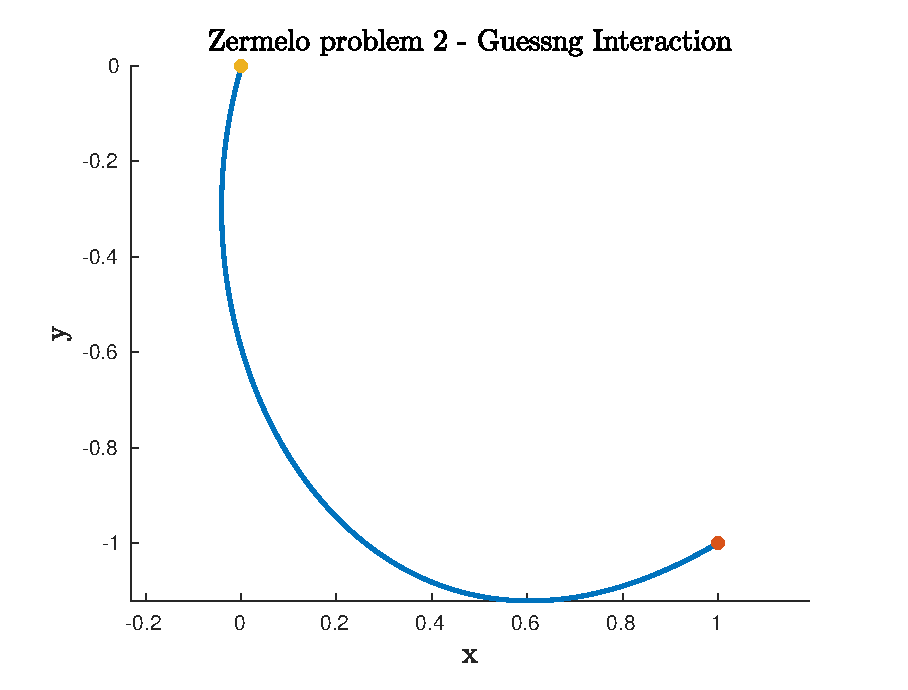
\includegraphics [width=4in]{f3}
\caption{Zermelo's solution for x(0) = 1, y(0) = -1}
\end{figure}

\section{Minimum-Drag Nose Shape}

\begin{figure}[H]
\centering
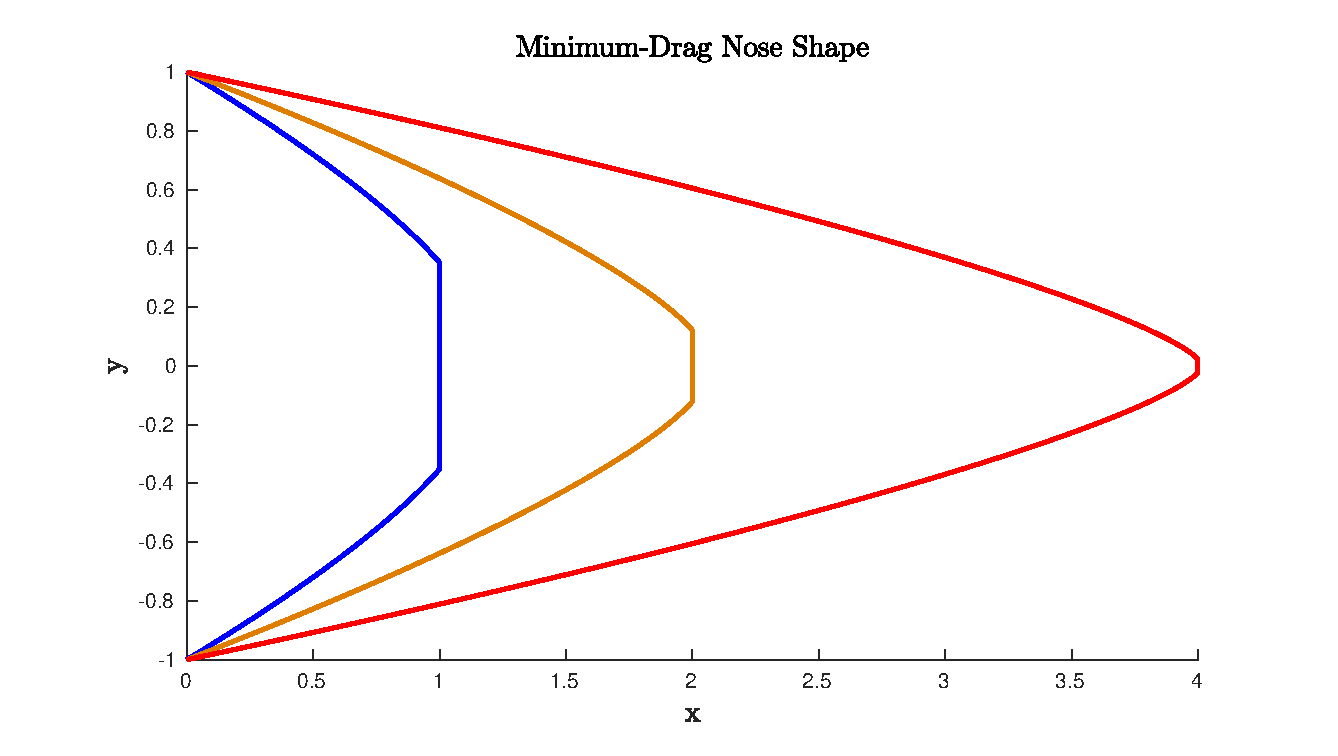
\includegraphics [width=4.4in]{f5}
\caption{Minimum-Drag Nose Shape for l=1,2,and 4}
\end{figure}

\section{Code}

\begin{lstlisting}
% Book: Optimal Control Theory: An introduxtion by Donald E. Kirk
% 
% Erivelton Gualter, 03/19/2018

%% PROBLEM 1 %%%%%%%%%%%%%%%%%%%%%%%%%%%%%%%%%%%%%%%%%%%%%%%%%%%%%%

clear all; clc; close all

% Boundary Conditions
xo = 3.66;  
yo = -1.86;
xf = 0;     
yf = 0;

ts = 0.01;         % Sampling time
q = 0:0.001:2*pi;   % angle guess array
t = 0:ts:10;       % Array time

Z = zeros(length(t),3); % Initialize states
minimum = Inf;          % Variable to find the best gues

% Brush the angle array to find the best angle guess
for j=1:length(q)
    Z(1,:) = [ xo yo q(j)]; % Initial state condition
    
    % Euler Integration
    for i=1:length(t)-1 

        % Load states
        z1 = Z(i,1);
        z2 = Z(i,2);
        z3 = Z(i,3);

        % Dot States
        z1d = cos(z3)-z2;
        z2d = sin(z3);
        z3d = cos(z3)^2;

        Zdot = [z1d z2d z3d];

        % Integration
        Z(i+1,:) = Z(i,:) + Zdot*ts; 

        % Euclidian distance of the final position to [xf yf]
        best = norm(Z(i+1,1:2)-[xf yf]);
        if best < minimum
            minimum = best; % Update minimum flag
            
            Zopt = Z;           % Final States
            topt = t(1:i);      % time array
            Zopt = Zopt(1:i,:); 
            tfinal = t(i); 
        end
    end
end

% Find the angles using the guess condition
syms theta thetaf
sol = vpasolve([yo == sec(theta) - sec(thetaf), ...
                xo == -(sec(thetaf)*(tan(thetaf)-tan(theta)) - ...
                tan(theta)*(sec(thetaf)-sec(theta)) + ...
                log((tan(thetaf)+sec(thetaf))/(tan(theta)+sec(theta))))/2] ...
                ,[theta thetaf],[Zopt(1,3) Zopt(end,3)]); %[2.6270 1.2935]);
            
Z(1,:) = [ xo yo double(sol.theta)]; % Initial condition
% Euler Integration Method
for i=1:length(t)-1

    % Load states
    z1 = Z(i,1);
    z2 = Z(i,2);
    z3 = Z(i,3);

    % Dot States
    z1d = cos(z3)-z2;
    z2d = sin(z3);
    z3d = cos(z3)^2;

    Zdot = [z1d z2d z3d];

    % Integration
    Z(i+1,:) = Z(i,:) + Zdot*ts; 
end
    
f1 = figure; hold on;
plot(Zopt(:,1), Zopt(:,2),'LineWidth',2);
plot(xo, yo, '*','LineWidth',2);
plot(xf, yf, '*','LineWidth',2);
axis equal

title('Zermelo problem 1', 'Interpreter','Latex', 'FontSize',14);
xlabel('x', 'Interpreter','Latex', 'FontSize',14);
ylabel('y', 'Interpreter','Latex', 'FontSize',14);

saveFigureToPdf('f1', f1)

%% PROBLEM 2 %%%%%%%%%%%%%%%%%%%%%%%%%%%%%%%%%%%%%%%%%%%%%%%%%%%%%%

clear all; clc; 

% Boundary Conditions
xo = 1;  
yo = -1;
xf = 0;     
yf = 0;

ts = 0.01;          % Sampling time
topt = 0:ts:10;     % Array time
q = 0:0.001:2*pi;   % angle time

Z = zeros(length(topt),3);
minimum = Inf;

% Euler integration for q=0:2pi
for j=1:length(q)
    Z(1,:) = [ xo yo q(j)]; % Load initial condition
    
    for i=1:length(topt)-1

        % States
        z1 = Z(i,1);
        z2 = Z(i,2);
        z3 = Z(i,3);

        % Derivative states
        z1d = cos(z3);
        z2d = sin(z3)-z1;
        z3d = -sin(z3)^2;

        Zdot = [z1d z2d z3d];

        % Euler integration
        Z(i+1,:) = Z(i,:) + Zdot*ts;
        
        % Find best path to reach the final position
        best = norm(Z(i+1,1:2)-[xf yf]);
        if best < minimum
            minimum = best;
            Zopt = Z;
            tfidx = i;
            qo = q(j);
        end
    end
end

% reshape array 
topt = topt(1:tfidx);
Zopt = Zopt(1:tfidx,:);

% Plot
figure; hold on
plot(Zopt(:,1), Zopt(:,2),'LineWidth',2);
plot(xo, yo, '*','LineWidth',2);
plot(xf, yf, '*','LineWidth',2);
axis equal
title('Zermelo problem 2 - Guessng Interaction', 'Interpreter','Latex', 'FontSize',14);
xlabel('x', 'Interpreter','Latex', 'FontSize',14);
ylabel('y', 'Interpreter','Latex', 'FontSize',14);

% Find the angles using the guess condition
syms theta thetaf
sol2 = vpasolve([yo == csc(theta) - csc(thetaf), ...
                xo == -(csc(thetaf)*(cot(thetaf)-cot(theta)) - ...
                cot(theta)*(csc(thetaf)-csc(theta)) + ...
                log((cot(thetaf)+csc(thetaf))/(cot(theta)+csc(theta))))/2] ...
                ,[theta thetaf],[Zopt(1,3) Zopt(end,3)]);
            
Z(1,:) = [ xo yo double(sol2.theta)]; % Initial condition
for i=1:length(topt)-1

    % States
    z1 = Z(i,1);
    z2 = Z(i,2);
    z3 = Z(i,3);

    % Derivative states
    z1d = cos(z3);
    z2d = sin(z3)-z1;
    z3d = -sin(z3)^2;

    Zdot = [z1d z2d z3d];

    % Euler integration
    Z(i+1,:) = Z(i,:) + Zdot*ts;

    best = norm(Z(i+1,1:2)-[xf yf]);
    if best < minimum
        minimum = best;
        Zopt = Z;
        tfidx = i;
        qo = q(j);
    end
end

% Plots
figure; hold on
plot(Zopt(:,1), Zopt(:,2),'LineWidth',2);
plot(xo, yo, '*','LineWidth',2);
plot(xf, yf, '*','LineWidth',2);
axis equal
title('Zermelo problem 2 - Finding guess angle directly', 'Interpreter','Latex', 'FontSize',14);
xlabel('x', 'Interpreter','Latex', 'FontSize',14);
ylabel('y', 'Interpreter','Latex', 'FontSize',14);

%% PROBLEM 3 %%%%%%%%%%%%%%%%%%%%%%%%%%%%%%%%%%%%%%%%%%%%%%%%%%%%%%

clear all, clc

% Parameters of the problem
a = 1; 
l = 1; %1,2,4 
dx = 0.01;      % Sampling
x = 0:dx:l;     % array x

% Initialization of u and r
u = zeros(size(x));
r = zeros(size(x));

% At x=0
syms uo rl un rn

% Solve r and ul to the initial point
s1 = vpasolve([a == rl*(1+uo^2)^2/(4*uo^3), ...
               l == rl*((3/(4*uo^4) + 1/uo^2 - 7/4 + log(uo)))/4], ...
               [rl, uo], [0.3 0.5]);
      
% Convert results to double
u(1) = double(s1.uo);
r(1) = a;
rl = double(s1.rl);

% Solve u and r for deltaX
% At x= dx*x
for i=2:length(x)-1
    s2 = vpasolve([rn == rl*(1+un^2)^2 / (4*un^3), ...
                   rl == (l-(i-1)*dx)/ ((1/4)*(3/(4*un^4) + 1/un^2 - 7/4 + log(un)))], ...
                   [un, rn], [u(i-1) r(i-1)]);

    r(i) = double(s2.rn); % Convert to double
    u(i) = double(s2.un); % Convert to double
end

% Connect data
r(end) = rl;
x = [x l];
r = [r 0];

% Plots
hold on;
plot(x,r, x,-r,'b','LineWidth',2);
title('Minimum-Drag Nose Shape', 'Interpreter','Latex', 'FontSize',14);
xlabel('x', 'Interpreter','Latex', 'FontSize',14);
ylabel('y', 'Interpreter','Latex', 'FontSize',14);

\end{lstlisting}

You can access the code at: https://github.com/EriveltonGualter/EEC-744-Optimal-Control-Systems

\end{document}
